\subsection{Text-based retrieval augmented-generation}
\begin{figure}[hbt]
    \centering
    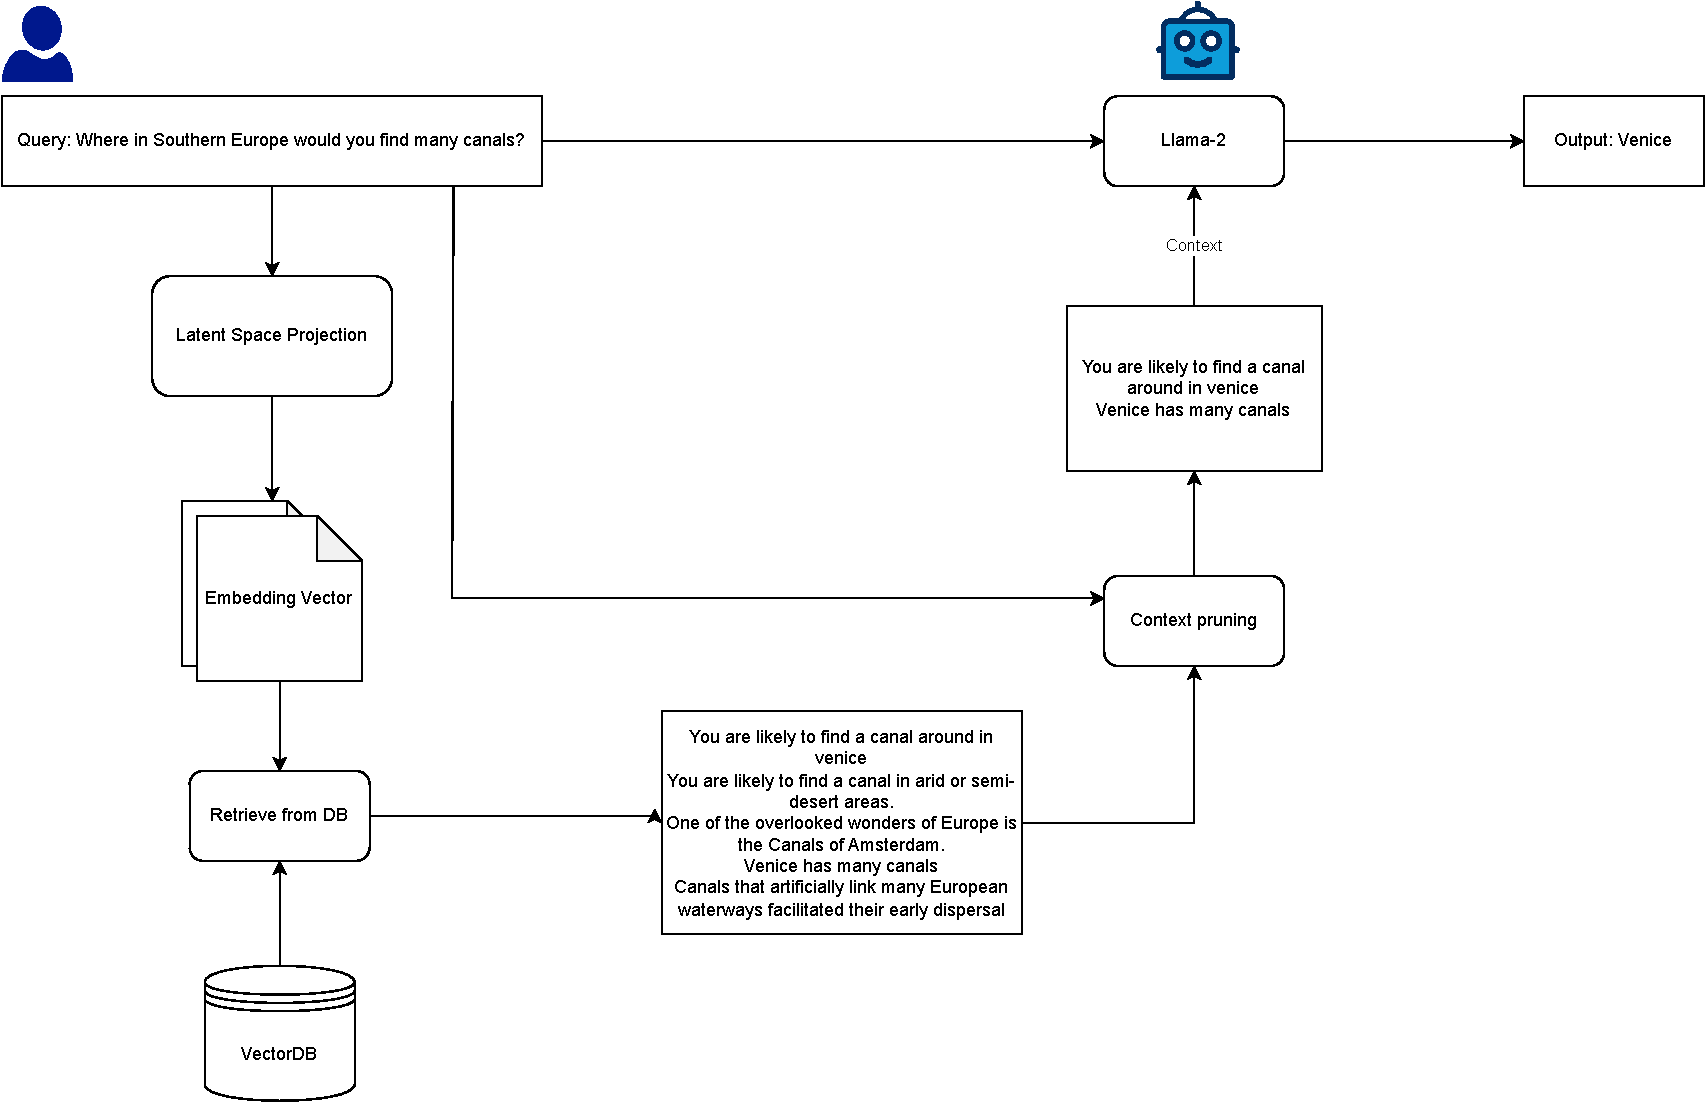
\includegraphics[width=0.95\linewidth]{experiements/image/rag.pdf}
    \caption{General 2-stage pipeline of retrieval-augmented generation}
    \label{fig:p_rag}
\end{figure}
Figure \ref{fig:p_rag} illustrated the pipeline of Retrieval-augmented generation. It includes \textit{Latent projection}, \textit{Retrieval}, \textit{Context pruning}, \textit{Generator}.\\
% Commonsense corpus includes about 20 million short sentences \cite{yu2022retrieval} relating various commonsense reasoning tasks.
\textbf{Preprocessing data:}  Knowledge base contains short sentences. Each sentence is projected to latent space by using Bi-encoder in order to construct vector database.

\textbf{Latent projection:} The Bi-encoder is employed to map the query from the user to the same latent space of documents in vector database.

\textbf{Retrieval:} In this phase, cosine similarity is used to compare between each embedding vector of documents in vector database and embedding vector of query to select top-K documents based on similarity score.

\textbf{Context pruning:} In this phase, the main objective is to perform reranking on the top-K documents after retrieval. This process helps to select the context documents more precisely and relevantly. The Cross-encoder is employed to compare the query with each top-K document. After that, top-K’ documents (where K’ $<$ K) are extracted and passed to the generator to generate the answer for the user.